\documentclass{standalone}
\usepackage{mintikz}

\begin{document}
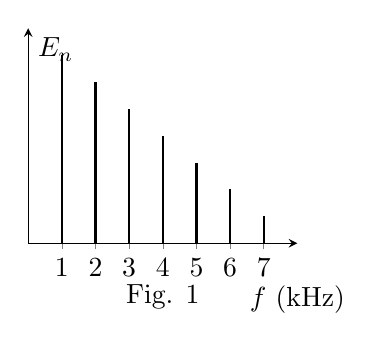
\begin{tikzpicture}[]
    \begin{axis}[
        xmin=0, xmax=8,
        ymin=0, ymax=8,
        xtick={1, 2, ..., 7},
        ytick=\empty,
        xlabel=$f$ (kHz), ylabel=$E_n$,
        axis lines=center,
        x label style={at={(axis description cs:1,-0.15)},anchor=north},
        width=5cm,
        clip=false]
        % \addplot[
        % domain=1:8,
        % smooth,
        % black]
        % {\x};
        \draw[thick]
        (axis cs:1, 0) --
        (axis cs:1, 7)
        (axis cs:2, 0) --
        (axis cs:2, 6)
        (axis cs:3, 0) --
        (axis cs:3, 5)
        (axis cs:4, 0) --
        (axis cs:4, 4)
        (axis cs:5, 0) --
        (axis cs:5, 3)
        (axis cs:6, 0) --
        (axis cs:6, 2)
        (axis cs:7, 0) --
        (axis cs:7, 1)
        ;
        \node[] at (axis cs:4,-2) {Fig. 1};
    \end{axis}
\end{tikzpicture}
\hspace{.2cm}
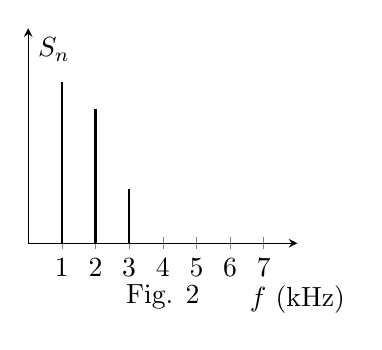
\begin{tikzpicture}[]
    \begin{axis}[
        xmin=0, xmax=8,
        ymin=0, ymax=8,
        xtick={1, 2, ..., 7},
        ytick=\empty,
        xlabel=$f$ (kHz), ylabel=$S_n$,
        axis lines=center,
        x label style={at={(axis description cs:1,-0.15)},anchor=north},
        width=5cm,
        clip=false]
        % \addplot[
        % domain=1:8,
        % smooth,
        % black]
        % {\x};
        \draw[thick]
        (axis cs:1, 0) --
        (axis cs:1, 6)
        (axis cs:2, 0) --
        (axis cs:2, 5)
        (axis cs:3, 0) --
        (axis cs:3, 2)
        (axis cs:4, 0) --
        (axis cs:4, 0)
        (axis cs:5, 0) --
        (axis cs:5, 0)
        (axis cs:6, 0) --
        (axis cs:6, 0)
        (axis cs:7, 0) --
        (axis cs:7, 0)
        ;
        \node[] at (axis cs:4,-2) {Fig. 2};
    \end{axis}
\end{tikzpicture}
\hspace{.2cm}
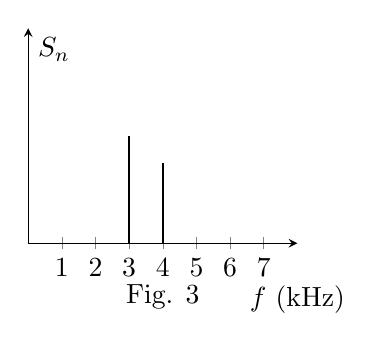
\begin{tikzpicture}[]
    \begin{axis}[
        xmin=0, xmax=8,
        ymin=0, ymax=8,
        xtick={1, 2, ..., 7},
        ytick=\empty,
        xlabel=$f$ (kHz), ylabel=$S_n$,
        axis lines=center,
        x label style={at={(axis description cs:1,-0.15)},anchor=north},
        width=5cm,
        clip=false]
        % \addplot[
        % domain=1:8,
        % smooth,
        % black]
        % {\x};
        \draw[thick]
        (axis cs:1, 0) --
        (axis cs:1, 0)
        (axis cs:2, 0) --
        (axis cs:2, 0)
        (axis cs:3, 0) --
        (axis cs:3, 4)
        (axis cs:4, 0) --
        (axis cs:4, 3)
        (axis cs:5, 0) --
        (axis cs:5, 0)
        (axis cs:6, 0) --
        (axis cs:6, 0)
        (axis cs:7, 0) --
        (axis cs:7, 0)
        ;
        \node[] at (axis cs:4,-2) {Fig. 3};
    \end{axis}
\end{tikzpicture}
\hspace{.2cm}
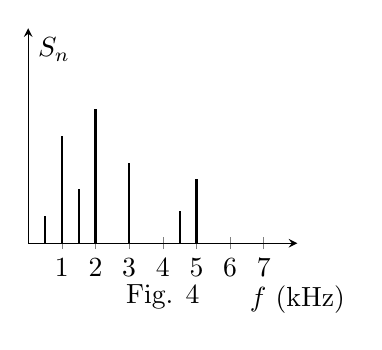
\begin{tikzpicture}[]
    \begin{axis}[
        xmin=0, xmax=8,
        ymin=0, ymax=8,
        xtick={1, 2, ..., 7},
        ytick=\empty,
        xlabel=$f$ (kHz), ylabel=$S_n$,
        axis lines=center,
        x label style={at={(axis description cs:1,-0.15)},anchor=north},
        width=5cm,
        clip=false]
        % \addplot[
        % domain=1:8,
        % smooth,
        % black]
        % {\x};
        \draw[thick]
        (axis cs:0.5, 0) --
        (axis cs:0.5, 1)
        (axis cs:1, 0) --
        (axis cs:1, 4)
        (axis cs:1.5, 0) --
        (axis cs:1.5, 2)
        (axis cs:2, 0) --
        (axis cs:2, 5)
        (axis cs:3, 0) --
        (axis cs:3, 3)
        (axis cs:4, 0) --
        (axis cs:4, 0)
        (axis cs:4.5, 0) --
        (axis cs:4.5, 1.2)
        (axis cs:5, 0) --
        (axis cs:5, 2.4)
        (axis cs:6, 0) --
        (axis cs:6, 0)
        (axis cs:7, 0) --
        (axis cs:7, 0)
        ;
        \node[] at (axis cs:4,-2) {Fig. 4};
    \end{axis}
\end{tikzpicture}
\end{document}
